\documentclass[a4paper, 14pt]{extreport}
\pagestyle{plain}

\usepackage[T1, T2A]{fontenc}	
\usepackage[english,russian]{babel} %Русские шрифты
\usepackage[utf8]{inputenc}

\usepackage{extsizes} % вроде бы для размера шрифтов

\usepackage{graphicx} % для вставки картинок
\usepackage{gensymb} % нужен символ градуса
\usepackage{amssymb,amsfonts,amsmath,amsthm,mathrsfs} % математические дополнения от АМС
\usepackage{hyperref} %для гиперссылок
\usepackage{indentfirst} %отступ для первой главы параграфа
\usepackage{upgreek} %для красивенькой буквы фи
\usepackage{listings} % для листинга кода
\usepackage{color} % для использоания цветного фона в листинге кода
%\usepackage[justification=centering]{caption}  % для центрирования подписи в картинке
\usepackage{subcaption}
\usepackage{tocloft} % для нормального размера названия заголовка содержания
\usepackage{caption} % для человеческих подписей к рисункам
\usepackage{titlesec}
\usepackage{titletoc}
\usepackage[style=russian]{csquotes} % угловые кавычки
\usepackage{float} % для нормального позиционирования картинок


\usepackage{geometry} % отступы и все такое
 \geometry{
 a4paper,
 left=30mm,
 right=10mm,
 top=20mm,
 bottom=20mm,
 } 

\unitlength=1mm %Единица измерения длины в рисунках - 1 мм
\renewcommand{\bfdefault}{b}   % Делает жирный шрифт менее широким	
\renewcommand{\Re}{\text {Re}}
\renewcommand{\Im}{\text {Im}}
\renewcommand{\baselinestretch}{1.5} % межстрочный интервал
\setcounter{page}{3} % старт номера страниц

\setcounter{tocdepth}{3} % subsubsection в оглавлении

\makeatletter
\renewcommand\@biblabel[1]{#1.} % нормальная нумерация источником
\makeatother

\setlength{\cftbeforetoctitleskip}{-3em}

\titlecontents{chapter}
[0pt]
{}
{\contentsmargin{0pt}
    \thecontentslabel\enspace}
{\contentsmargin{0pt}\normal}
{\titlerule*[.5pc]{.}\contentspage}
[]

\lstset{ %настроки листинга кода. чтобы красивенько было, вот это вот все
	language=Python,
	keepspaces=true,
	numbers=left,
	linewidth=15cm,
	frame=L,
	basicstyle=\footnotesize,
	showstringspaces=false,
	inputencoding=utf8,
	extendedchars=\true
}

%change semicolon to defis in pictures:
\RequirePackage{caption}
\DeclareCaptionLabelSeparator{defffis}{ -- }
\captionsetup{justification=centering, labelsep=defffis}

% отступ в заголовках
\newlength{\normalparindent}
\AtBeginDocument{}
\titleformat{name=\section}[block]
  {\Large\bfseries}
  {\hspace{\normalparindent}\thesection}
  {0.5em}
  {}
	
% отступ в подзаголовках
\titleformat{name=\subsection}[block]
  {\large\bfseries}
  {\hspace{\normalparindent}\thesubsection}
  {0.5em}
  {}
	
% отступ в подподзаголовках	
\titleformat{name=\subsubsection}[block]
	{\bfseries}
	{\hspace{\normalparindent}\thesubsubsection}
  {0.5em}
  {}

% chapters format
\titleformat{\chapter}[display]   
{\normalfont\huge\bfseries\center}
{\chaptertitlename\ \thechapter}
{0pt}
{\huge}   
\titlespacing*{\chapter}{0pt}{-50pt}{0pt}


\AtBeginDocument{
   \let\div\relax % чтобы операторы дивергенции и градиента чуть что красивенько писались
   \DeclareMathOperator{\div}{div}
          \DeclareMathOperator{\grad}{grad}
          \setlength{\normalparindent}{\parindent} % для выравнивания заголовков
}


% шрифты на linux более гладкие
\pdfpkmode{dpdfezzz}
\pdfpkresolution=8000

\begin{document}
\renewcommand{\figurename}{Рисунок} % чтобы рисунки назывались не "Рис.", а "Рисунок", должно быть под Russian, ибо собьется
\renewcommand{\contentsname}{\hfill\Large ОГЛАВЛЕНИЕ \hfill}
\renewcommand{\cftaftertoctitle}{\hfill}




\begin{titlepage}
    \begin{center}
        \normalsize {\bf МИНИСТЕРСТВО ОБРАЗОВАНИЯ РЕСПУБЛИКИ БЕЛАРУСЬ} \\
        \vspace{0.5cm}
        \normalsize {\bf БЕЛОРУССКИЙ ГОСУДАРСТВЕННЫЙ УНИВЕРСИТЕТ} \\
        \vspace{0.5cm}
        \normalsize {\bf Факультет прикладной математики и информатики} \\
        \vspace{0.5cm}
        \normalsize {\bf Кафедра математического моделирования и управления} \\
        \vspace{2cm}
        КОЗЛЕНКОВ \\
        Алексей Андреевич \\
        \vspace{1cm}
        \normalsize {\bf ЧИСЛЕННОЕ РЕШЕНИЕ ГРАНИЧНОЙ ЗАДАЧИ ДЛЯ УРАВНЕНИЙ ТЕОРИИ УПРУГОСТИ МЕТОДОМ
        КОНЕЧНЫХ ЭЛЕМЕНТОВ}\\
        \vspace{1cm}
        \normalsize Дипломная работа \\
        \vspace{2cm}
        \begin{tabbing}
            MMMMMMMMMMMMMMMMMMMMMMMM \= MMMMMMM \kill
            \> Руководитель: \\
            \>  кандидат физ.-мат. наук, \\
            \> доцент Лемешевский С.В. 
        \end{tabbing}
        \begin{tabbing}
            MMMMMMMMMMMMMMMMMMMMMMMMM \= MMMMMMM \kill
            Допустить к защите \>  \\
            с предварительной оценкой \underline{\hspace{0.5cm}} \\
            <<\underline{\hspace{1cm}}>> \underline{\hspace{3.3cm}} 2017 г.
        \end{tabbing}

        \vspace{2cm}

        \large Минск, 2017
    \end{center}
    
\end{titlepage}

\clearpage
\setcounter{page}{2}

\tableofcontents



\newpage
\phantomsection
\begin{center}
	\Large{\textbf{РЕФЕРАТ}}
\end{center}

Дипломная работа, 37 страниц, 16 рисунков, 3 источника, 1 приложение.

\textbf{\textit{Ключевые слова:}} ТЕОРИЯ УПРУГОСТИ, МЕТОД КОНЕЧНЫХ 
ЭЛЕМЕНТОВ, ТЕНЗОР НАПРЯЖЕНИЯ, ТЕНЗОР ДЕФОРМАЦИИ, PYTHON, FEniCS, 
GMSH, PARAVIEW.

\textbf{\textit{Объект исследования:}} граничная задача теории 
упругости в области сложной формы.

\textbf{\textit{Цель работы:}} реализовать метод приближенного решения
задачи теории упругости в рассматриваемой области с помощью пакета
\texttt{FEniCS}, провизуализировать и проанализировать результаты.

\textbf{\textit{Методы исследования:}} метод конечных элементов.

\textbf{\textit{Результат:}} сценарий на языке \texttt{Python},
использующий возможности пакета \texttt{FEniCS}.

\textbf{\textit{Область применения:}} численные решения краевых 
дифференциальных задач эллиптического типа в частных производных.

\begin{center}
	\Large{\textbf{РЭФЕРАТ}}
\end{center}

Дыпломная праца, 37 старонак, 16 малюнкаў, 3 крыніцы, 1 дадатак.

\textbf{\textit{Ключавыя словы:}} ТЕОРИЯ ПРУГКАСЦІ, МЕТАД КАНЧАТКОВЫХ \\
ЭЛЕМЕНТАЎ, ТЭНЗАР НАПРУГКАСЦI, ТЕНЗАР ДЭФАРМАЦЫІ, PYTHON, \\ FEniCS, 
GMSH, PARAVIEW.

\textbf{\textit{Аб'ект даследавання:}} межавая задача тэорыі 
пругкасці ў вобласці складанай формы.

\textbf{\textit{Мэта работы:}} пабудаваць метад для колькаснага 
рашэння задачы теорыі пругкасці ў расгледжваемай вобласці з
дапамогай пакета \texttt{FEniCS}, правiзулiзаваць и прааналізіраваць вынікі.

\textbf{\textit{Метады даследавання:}} метад канчатковых элементаў.

\textbf{\textit{Вынiкi:}} праграма на мове \texttt{Python},
якая выкарыстоўвае магчамасці пакета \texttt{FEniCS}.

\textbf{\textit{Вобласць выкарыстання:}} колькасныя рашэнні мэжавых 
дыфференцыяльных задач эліптычнага тыпу ў прыватных вытворных.


\begin{center}
	\Large{\textbf{SUMMARY}}
\end{center}

Diploma paper, 37 pages, 16 pictures, 3 sources, 1 appendix.

\textbf{\textit{Keywords:}} ELASTICITY THEORY, FINITE ELEMENT METHOD,
STRESS TENSOR,  STRAIN TENSOR, PYTHON, FEniCS, GMSH, 
PARAVIEW.

\textbf{\textit{Research object:}} boundary problem of the elasticity
theory in complex domain.

\textbf{\textit{Purpose:}} to build a method for numerical solving 
elasticity theory problem in current domain using the \texttt{FEniCS}
package and to visualize and analyze the results.

\textbf{\textit{Research methods:}} the finite element method.

\textbf{\textit{Result:}} Python script which use \texttt{FEniCS}
package abilities.

\textbf{\textit{Application field:}} numerical solving of the
boundary problems for partial differential equations of the elliptic type.


\newpage
\phantomsection
\begin{center}
\addcontentsline{toc}{section}{ВВЕДЕНИЕ}
	\Large{\textbf{ВВЕДЕНИЕ}}
\end{center}

В настоящее время информационные технологии все сильнее 
проникают в самые различные области медицины, в том числе в 
стоматологию. И речь идет не о банальном использовании 
компьютера как пишущей машинки. Компьютерные 
мощности активно используются на этапах диагностики: 
сканированные диагностические модели, цифровая рентенография и фотография, и протезирования.

Для обоснования различных типов протезирующих конструкций 
широко используются методы математического моделирования.
Суть их заключается в прогнозировании результатов врачебного 
вмешательства при расчетах напряженно-деформированных 
состояний органов зубочелюстной системы, протезов или 
коронок. В данной работе речь пойдет о телескопических
коронках.
Существует несколько различных вариантов конструкций
телескопических (состоящих из нескольких частей) коронок 
как удерживающих элементов для съемных протезов.
Одним из них является конструкция, основанная на 
цилиндрах. Однако, при таком подходе между соединениями
происходит параллельное соединение, при котором, с момента 
первого контакта поверхностей и до полного наложения, 
происходит динамическое трение, что вызывает 
преждевременное стирание поверхностей элементов. То 
же происходит и при разъединении составляющих.
Конусовидные коронки лишены этого недостатка: когда конус
помещается в соответствующий ему вогнутый конус, сцепление
возникает только в конечном положении, что предотвращает 
преждевременное изнашивание элементов конструкции.


Расчетом напряженно-деформированного состояния 
твердых тел занимается теория упругости. Задачи теории
упругости, как и множество других задач, сводящиеся к
уравнениям в частных производных, зачастую трудно 
разрешимы аналитическим способом, например, по причине
неординарной формы области. Посему, для решения таких
задач широко используются численные методы.

Метод конечных элементов \cite{finite_element_method} -- это численный метод, 
предназначенный также для решен-ия 
дифференциальных уравнений в частных производных, 
возникающих при решении задач математической физики. 
Метод широко используется для решения задач механики 
деформируемого твёрдого тела, а также для задач теплообмена, 
гидродинамики и электродинамики.
Как следует из названия метода, суть его заключается в поиске 
решения на дискретизированной области -- разбиении 
оригинальной области на множество подобластей (элементов).
Для каждого элемента выбирается вид аппроксимирующей
функции (в простейшем случае -- полином 1-й степени).
Эти функции равны нулю вне области своего элемента.
Также соблюдаются условия согласования -- равенство
значений  аппроксимирующих функций на границах элементов
 (в узлах). 
Эти условия согласования также позволяют определить 
коэффициенты аппроксимирующих функций на своих элементах.
Составляется и решается система алгебраических уравнений.
Так как каждая функция ограничена областью своего элемента, 
система обычно получается разреженной, что упрощает ее 
решение.
Метод конечных элементов имеет несколько преимуществ 
по сравнению со свои ближайшим аналогом -- методом 
конечных разностей (МКР): МКЭ позволяет работать с более 
сложными областями; также найденная функция сразу является 
решением -- при использовании МКР еще нужно построить
сплайн (или другую интерполяцию).

В данной работе проводится моделирование напряжений 
для телескопических конусовидных коронок.

В первой главе дается описание исследуемой задаче, 
приводится постановка в дифференциальной формулировке.

Во второй главе описана аппроксимация задачи методом
конечных элементов.

Третья глава посвящена описанию процесса моделирования, 
визуализации и анализу результатов.


\chapter{Постановка задачи теории упругости}
\section{Формулировка задачи}
\subsection{Общая формулировка задачи теории упругости}


Под влиянием приложенных сил твердые тела могут изменять свои форму и объем, 
т.е. в той или иной степени деформироваться.

Пусть радиус-вектор \, $\textbf{x} = (x_1, x_2, x_3)$ \, описывает координаты 
некоторой материальной точки твердого тела до воздействия на него внешних сил,
а \, $\textbf{x}' = (x'_1, x'_2, x'_3)$ \, -- радиус вектор той же материальной
точки после действия внешних сил. Перемещение точки характеризуется 
\textit{вектором упругих деформаций} \,$\textbf{u} = \textbf{x}' - \textbf{x}$, 
где  $u_i = x'_i - x_i$. Деформированное состояние тела
полностью описывается заданием вектора упругих деформаций для каждой точки тела.

Задача \texttt{теории упругости} (\cite{math_elasticity_theory}) состоит в 
отыскании вектора $\textbf{u}$ как функции, исходя из начальных условий.

\subsection{Описание рассматриваемой задачи}

Рассмотрим задачу для трехмерной области сложной формы, диаметральное сечение
которой представлено на рисунке \ref{fig: domain}.
\begin{figure}[h]
	\center
	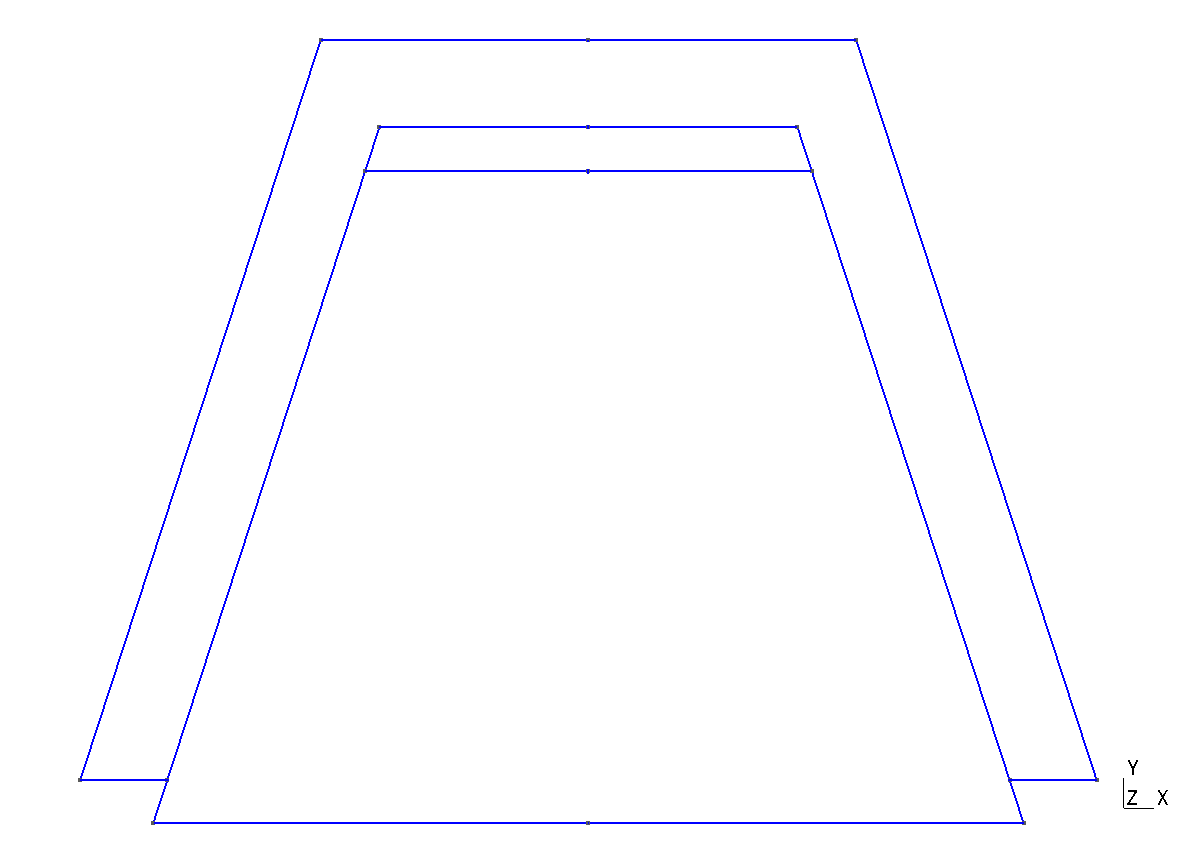
\includegraphics[scale=0.3]{pictures/1.png}
	\caption{Диаметральное сечение области}
	\label{fig: domain}
\end{figure}

Область представляет собой пару усеченных конусов, один из которых
\enquote{надет} на другой. Между конусами имеется свободное пространство (зазор).

К верхнему основанию внешнего конуса в некоторой
точке прикладывается нагрузка $\textbf{g}$
под некоторым углом.

Требуется определить, во-первых, напряженно-деформированное состояние тела после действия нагрузки, то есть решить основную задачу теории упругости.

Во-вторых, в качестве дополнительного исследования, будем оценивать состояние кумулятивной области на границе сопряжения составляющих областей после действия нагрузки и анализировать, проявилось ли смещение.

Такое моделирование в реальной жизни может быть применено к
процессу коронирования зубов, когда коронка относится к 
классу телескопических -- т.е. состоящих из нескольких 
элементов. Более подробное описание будет дано в
 \hyperref[ch:exp]{Главе 3}.



\section{Постановка задачи в дифференциальной форме}

Рассмотрим на диаметральном сечении основные части нашей области 
(рисунок \ref{fig: marked_domain}).
\begin{figure}[H]
	\center
	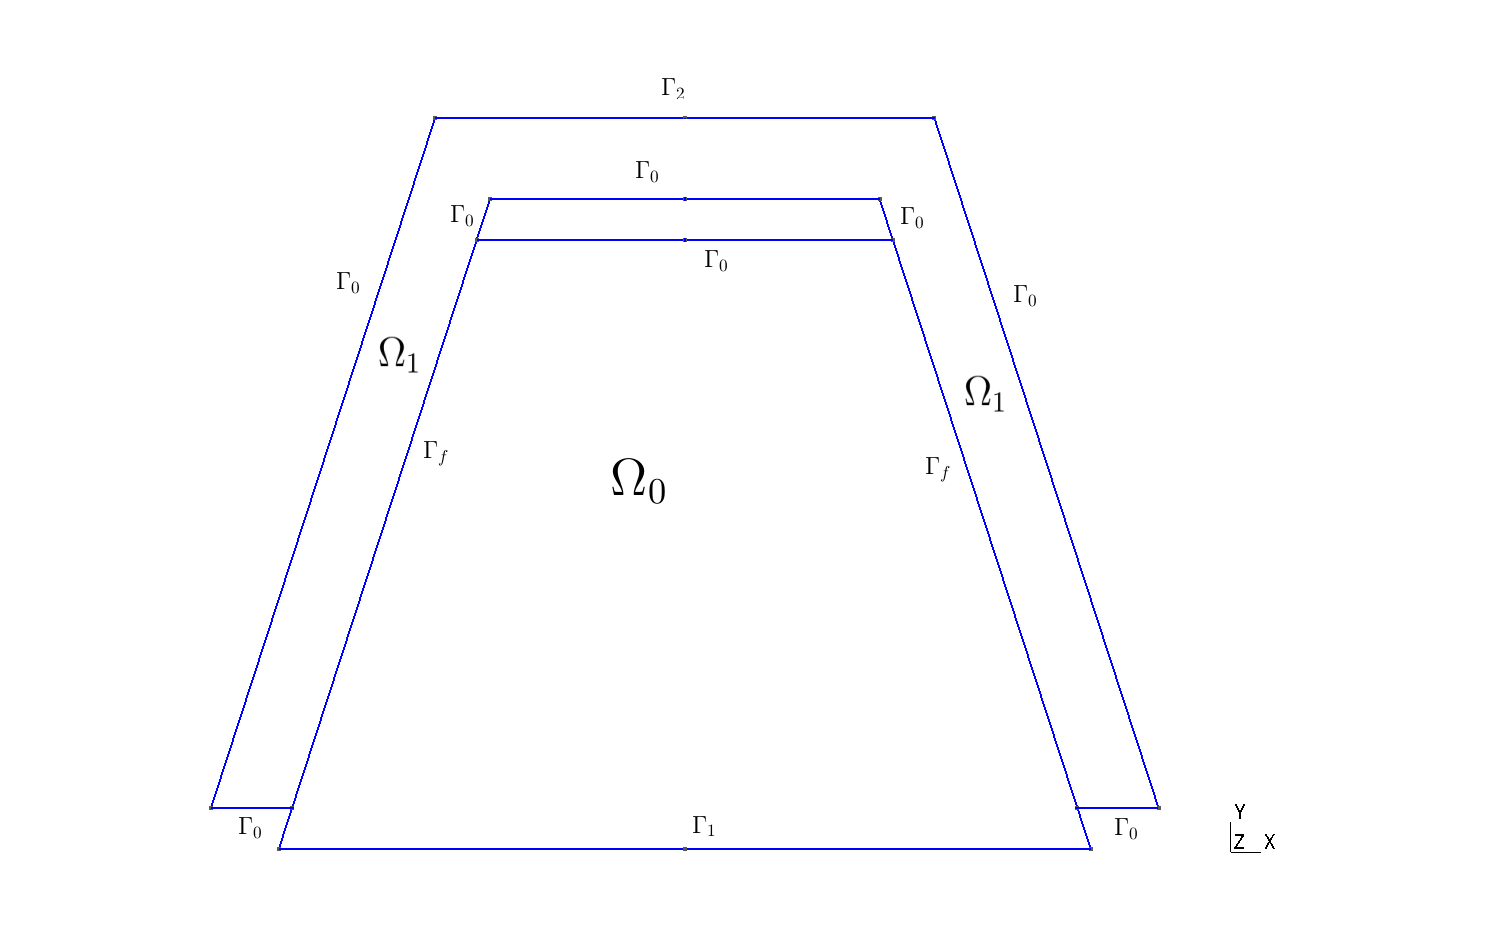
\includegraphics[scale=0.4]{pictures/marked_domain.png}
	\caption{Обозначение составляющих частей области (в разрезе)}
	\label{fig: marked_domain}
\end{figure}

Рассмотрим задачу в следующей дифференциальной формулировке:
\begin{equation}
	\label{eq:1}
	\nabla\!\cdot\!\sigma(\textbf{u}) = \textbf{0}, \textbf{x} \in \Omega = \Omega_0 \cup \Omega_1
\end{equation}
с граничными условиями:
\begin{equation}
	\label{eq: boundary_conditions}
	\begin{aligned}
		(\sigma(\textbf{u}), \textbf{n})(\textbf{x}) 	  	  &= \textbf{0},   &&\textbf{x} \in \Gamma_0,\\
		(\sigma(\textbf{u}), \textbf{n}) 				  	  &= \textbf{g},   &&\textbf{x} \in \Gamma_2, \; \textbf{g} = (g_1, g_2, g_3)\\
		\textbf{u}(\textbf{x})							  	  &= \textbf{0},	   &&\textbf{x} \in \Gamma_1,\\
		(\sigma(\textbf{u}), \textbf{n})\vert_{\Gamma_{f - 0}} &= 
			(\sigma(\textbf{u}), \textbf{n})\vert_{\Gamma_{f + 0}},             &&\textbf{x} \in \Gamma_f,
	\end{aligned}
\end{equation}
где $\sigma(\textbf{u})$  -- \texttt{тензор напряжений}, \textbf{n} -- вектор нормали
к поверхности. 

Граничные условия (\ref{eq: boundary_conditions}) означают, что к части поверхности 
$\Gamma_2$ приложена нагрузка, часть поверхности $\Gamma_1$ жестко закреплена, 
а на части поверхности $\Gamma_f$ выполняются условия сопряжения: напряжения 
с одной стороны поверхности противоположны по направлению напряжениям с 
другой стороны и равны по модулю.

Такая постановка задачи также называется \textit{постановкой в напряжениях}.

Известна связь между тензором напряжений $\sigma(\textbf{u})$ и \texttt{тензором деформаций}
$\varepsilon(\textbf{u}) = \frac{1}{2}(\nabla\textbf{u} + (\nabla\textbf{u}^T))$:
\begin{equation*}
\sigma(\textbf{u}) = \lambda \nabla\!\cdot\!\textbf{u}\textit{I} + 2\mu\varepsilon(\textbf{u})
\end{equation*}
где \textit{I} -- единичный тензор второго ранга,
$\lambda, \mu $ \, -- \texttt{коэффициенты Ламе}, также называемые 
\texttt{модулями упругости}, которые характеризуют упругие свойства тела. Заметим, что коэффициент $\mu$ также называется \texttt{модулем сдвига}. Они могут быть выраже­ны через модуль Юнга $E$ и коэффициент Пуассона $\nu$:
\begin{equation}
	\label{eq: young_puasson}
\mu = \frac{E}{2(1 + \nu)}, \quad \lambda = \frac{2\nu E}{(1 + \nu)(1 - 2\nu)}.
\end{equation}


Отсюда  можно получить формулировку (\ref{eq:1}) в \textit{перемещениях} (в векторной форме):
\begin{equation}
	\label{eq: 2}
	\mu\Delta\textbf{u} + (\lambda + \mu)\grad\!\nabla\!\cdot\!\textbf{u} = \textbf{0}
\end{equation}

\chapter{Аппроксимация задачи теории упругости методом конечных элементов}

Проведем аппроксимацию поставленной задачи методом
конечных элементов.
\section{ Вариационная формулировка}
При построении дискретной задачи для решения ее методом конечных элементов 
используется вариационная формулировка исходной дифференциальной задачи.
Опишем ее.

Введем следующие функциональные пространства:
\begin{itemize}
	\item $V = \{ \textbf{u(\textbf{x})} \in \textbf{H}^1(\Omega) \vert \textbf{u(\textbf{x})} = \textbf{0}, \textbf{x} \in \Gamma_1 \}$ --
	пространство \textit{триальных} функций;
	\item $\hat{V} = \{ \textbf{v(\textbf{x})} \in \textbf{H}^1(\Omega) \vert \textbf{v(\textbf{x})} = \textbf{0}, \textbf{x} \in \partial\Omega \}$ --
	пространство \textit{тестовых} функций.	
\end{itemize}

Для начала, скалярно домножим (\ref{eq:1}) на тестовую функцию $\textbf{v} \in \hat{V}$, 
а затем проинтегрируем по области $\Omega$.

По свойствам оператора дивергенции,
\begin{equation}
	\label{eq: 3}
	\nabla\!\cdot\!(\sigma(\textbf{u}), \textbf{v}) = (\textbf{v}, \nabla\!\cdot\!\sigma(\textbf{u})) +
		(\sigma(\textbf{u}), \nabla\textbf{v})
\end{equation}

Следовательно,
\begin{equation}
	\label{eq: 4}
	0 = \int\limits_\Omega{(\nabla\!\cdot\!\sigma(\textbf{u}), \textbf{v})}d\textbf{x} = 
		\int\limits_\Omega{\nabla\!\cdot\!(\sigma(\textbf{u}), \textbf{v})}d\textbf{x} - 
		\int\limits_\Omega{(\sigma(\textbf{u}), \nabla \textbf{v})}d\textbf{x}
\end{equation}

К первому слагаемому (\ref{eq: 4}) применим формулу Грина:
\begin{equation}
	\label{eq: 5}
	\begin{aligned}
		& \int\limits_\Omega{\nabla\!\cdot\!(\sigma(\textbf{u}), \textbf{v})}d\textbf{x} = 
		\int\limits_{\Omega_0}{\nabla\!\cdot\!(\sigma(\textbf{u}), \textbf{v})}d\textbf{x} \; +  \;
		\int\limits_{\Omega_1}{\nabla\!\cdot\!(\sigma(\textbf{u}), \textbf{v})}d\textbf{x} = \\
		& = \int\limits_{\partial\Omega_0}{((\sigma(\textbf{u}), \textbf{v}), \textbf{n})}dS + 
		\int\limits_{\partial\Omega_1}{((\sigma(\textbf{u}), \textbf{v}), \textbf{n})}dS = \\
		& = \int\limits_{\Gamma_2}{((\sigma(\textbf{u}), \textbf{v}), \textbf{n})}dS + 
		\int\limits_{\Gamma_f}{((\sigma(\textbf{u}), \textbf{n}_0) + (\sigma(\textbf{u}), \textbf{n}_1), \textbf{v})}dS + \\
		& + \int\limits_{\Gamma_0}{((\sigma(\textbf{u}), \textbf{v}), \textbf{n})}dS,
	\end{aligned}
\end{equation}
где $\textbf{n}_0$ и $\textbf{n}_1$ -- внешняя и внутренняя нормали к поверхности $\Gamma_f$,
т.е. они направлены в разные стороны, а значит, скалярные произведения с этими элементами 
отличаются лишь знаком, т.е. подынтегральное выражение интеграла по границе $\Gamma_f$ 
равно нулю.

Исходя из последнего утверждения, граничных условий и определения пространства $\hat{V}$,
(\ref{eq: 5}) преобразуется в:
\begin{equation}
	\label{eq: 6}
	\int\limits_\Omega{\nabla\!\cdot\!(\sigma(\textbf{u}), \textbf{v})}d\textbf{x} = 
	\int\limits_{\Gamma_2}{(\textbf{g}, \textbf{v})}dS
\end{equation}

Преобразовав подынтегральное выражение (\ref{eq: 4}) с учетом свойств тензоров, получим:
\begin{equation}
	\label{eq: 7}
	\int\limits_\Omega{(\sigma(\textbf{u}), \nabla \textbf{v})}d\textbf{x} = 
	\int\limits_{\Omega_0}{(\sigma(\textbf{u}), \varepsilon(\textbf{u}))}d\textbf{x} + 
	\int\limits_{\Omega_1}{(\sigma(\textbf{u}), \varepsilon(\textbf{u}))}d\textbf{x}
\end{equation}

В силу (\ref{eq: 6}) и (\ref{eq: 7}), (\ref{eq: 4}) преобразуется в:
\begin{equation}
	\label{eq: 8}
	\int\limits_{\Omega_0}{(\sigma(\textbf{u}), \varepsilon(\textbf{u}))}d\textbf{x} + 
	\int\limits_{\Omega_1}{(\sigma(\textbf{u}), \varepsilon(\textbf{u}))}d\textbf{x} = 
		\int\limits_{\Gamma_2}{(\textbf{g}, \textbf{v})}dS,
\end{equation}
что также можно записать в виде:
\begin{equation}
	\label{eq: 9}
	a(\textbf{u}, \textbf{v}) = L(\textbf{v}),
\end{equation}
где:
\begin{itemize}
	\item $a(\textbf{u}, \textbf{v}) : V \times \hat{V} \rightarrow \mathbb{R}$ \,-- \textit{билинейная форма};
	\item $L(\textbf{v}) : \hat{V} \rightarrow \mathbb{R}$ \, -- \textit{линейная форма}.
\end{itemize}

Задача состоит в том, чтобы отыскать такую  $\textbf{u} \in V$, 
которая удовлетворяет (\ref{eq: 9}).


\chapter{Рассчет напряжений в телескопических конусовидных коронках}
\label{ch:exp}

Проведем моделирование напряжений в телескопических
конусовидных коронках.


\section{Описание численного эксперимента}

Цель эксперимента -- оценить силу удержания конуса для рассматриваемой физической модели коронки.

Сила удержания возникает при прижимании коронок друг
к другу, внутренний конус входит как клин во внешний.  
При этом на поверхности конуса возникает значительная сила 
давления, которая направлена перпендикулярно поверхности -- 
нормальная сила, которая также определяет величину силы 
трения. Чем сильнее составные части коронки будут прижаты 
друг к другу, тем большая сила удержания возникнет и тем 
надежнее коронка будет зафиксирована.

Для того, чтобы оценить силу удержания, нужно по 
рассчитанному тензору напряжений
вычислить нормальные $f_n$ и тангенциальные 
$\boldsymbol{\tau}$ составляющие тензора. 
Вычислив нормальные и тангенциальные составляющие, мы 
можем, согласно закону Кулона-Амантона, оценить величину 
\texttt{силы удержания}:
\begin{equation}
	\label{eq: ka}
	f_{h} = k_0 f_n -|\boldsymbol{\tau}|,
\end{equation}
где $f_n$ -- нормальная составляющая тензора напряжений:
$$f_n = (-\boldsymbol{\sigma}, \boldsymbol{n}) \cdot \boldsymbol{n},$$
$\tau$ -- тангенциальная составляющая тензора напряжений:
$$\boldsymbol{\tau} = (-\boldsymbol{\sigma}, \boldsymbol{n}) - f_n \cdot \boldsymbol{n},$$
$k_0$ -- коэффициент трения скольжения (для заданных материалов ~0.15).

\subsection{Организация процесса вычислений}

В численном эксперименте будем производить несколько 
вариантов расчётов: для разных углов и для разных нагрузок. 
Углы будем варьировать в пределах от 
$4^{\circ}$ до $12^{\circ}$  с 
шагом 2. 

Среднестатистически, человеческая челюсть при жевании 
создает нагрузку порядка $10^8$ Па. 
Все варианты параметров численного эксперимента задаются в 
файле параметров \texttt{problem.xml}.

Генерировать область  и производить вычисления будем для 
каждой пары (угол-нагрузка) конкретного значения параметров.

Для генерации области и сетки будем использовать 
free-software пакет \texttt{Gmsh}.

Для проведения вычислений будем использовать open-source
инструмент \texttt{FEniCS} (\cite{fenics_book}), который 
предназначен  для решения методом конечных элементов  
задач, описываемых  уравнениями в частных производных. 

Для старта численного эксперимента используется файл \texttt{main.py}.
Данный скрипт, итерируясь по набору углов и набору заданных 
нагрузок, по шаблону \texttt{problem-template.xml} 
производит некоторые подготовительные действия:

\begin{itemize}
\item дополняет \texttt{problem.xml} конкретным значением нагрузки;
\item дополняет \texttt{problem.xml} необходимыми путями к файлам сетки, 
областей и файлам результатов;
\item дополняет \texttt{final.geo} необходимым параметром угла наклона
 образующей конуса;
\item запускает скрипт \texttt{meshgen.py} для генерации сетки;
\item запускает скрипт \texttt{elsasticity.py} для проведения самого 
эксперимента.
\end{itemize}

Для визуализации и анализа результатов будем использовать
свободно распространяемый  пакет \texttt{Paraview}.

\section{Построение области и сетки}

Одним из ключевых моментов в данной работе, как и при моделировании 
любой задачи математической физики, является построение области, 
на которой исследуется данная задача.

В данной работе для этой цели используется вышеупомянутый пакет
 \texttt{Gmsh}. С его помощью можно строить области различной формы
 путем объединения и преобразования простейших элементов в более 
 сложные (точки в линии, линии в контуры; контуры задают поверхности,
  поверхности -- объемы), а также генерировать сетку.

Для работы с формированием области используется файловый формат 
\texttt{.geo}, для сеток -- \texttt{.msh}.

\subsection{Формирование области}
\subsubsection{Геометрическое описание области моделирования}

Область, которая была проиллюстрирована на рисунке (\ref{fig: domain}),
можно построить, задав следующие параметры:
\begin{itemize}
	\item height -- высота внутреннего конуса;
	\item width -- радиус нижнего основания внутреннего конуса;
	\item $\alpha$ -- угол наклона образующей внутреннего конуса;
	\item space -- толщина \enquote{прослойки} между внутренним и внешним 
	конусами;
	\item border -- толщина внешнего конуса;
	\item delta -- расстояние между нижними основаниями конусов 
	(\enquote{высота} посадки внешнего конуса);
\end{itemize}

Используя эти параметры и математику 10 класса,
можно вычислить координаты всех опорных точек.

\subsubsection{Практическое моделирование области}

\texttt{Gmsh} предоставляет возможность очень четко и красиво,
 оперируя файлом \texttt{.geo} и своим графическим интерфейсом,  
формировать нужную область.
Файл \texttt{.geo} на самом деле представляет собой обычный текстовый файл, то есть в этом расширении нет никаких файловых особенностей.
Тот факт, что это обычный текстовый файл, дает возможность достаточно просто оперировать им из программного кода вычисляющего скрипта.

Вот так задаются параметры:
\begin{lstlisting}
DefineConstant[ alfa = { 4, Path "Gmsh/Parameters"}];
DefineConstant[ lc = { 0.0005, Path "Gmsh/Parameters"}];
DefineConstant[ height = { 0.012, Path "Gmsh/Parameters"}];
DefineConstant[ width = { 0.008, Path "Gmsh/Parameters"}];
DefineConstant[ space = { 0.001, Path "Gmsh/Parameters"}];
DefineConstant[ border = { 0.0015, Path "Gmsh/Parameters"}];
DefineConstant[ delta = { 0.001, Path "Gmsh/Parameters"}];
\end{lstlisting}

Также можно использовать некоторые, например, тригонометрические,
математические функции и константы:

\begin{lstlisting}
DefineConstant[ u_width = { width - height * 
	Tan(Pi*alfa / 180), Path "Gmsh/Parameters"}];
DefineConstant[ us_width = { width - (height + space) * 
	Tan(Pi*alfa / 180), Path "Gmsh/Parameters"}];
DefineConstant[ ub_width = { width - (height + space + border) * 
	Tan(Pi*alfa / 180), Path "Gmsh/Parameters"}];
DefineConstant[ l_width = { width - delta * 
	Tan(Pi*alfa / 180), Path "Gmsh/Parameters"}];
\end{lstlisting}

Точки задаются командой \texttt{Point}, которая, как и любой элемент в формируемой области,
отмечается уникальным номером и принимает 4 параметра: 3 пространственные 
координаты и величину, характеризующую масштаб сетки для ячеек рядом с этой точкой.

Линии задаются командами \texttt{Line} или \texttt{Circle},
в зависимости от формы линии.

Поверхности определяются контуром, составленным из
линий -- \texttt{Line Loop}. Поверхности также могут быть
плоскими -- \texttt{Plane Surface}, или изогнутыми --
\texttt{Ruled Surface}.

Аналогично определяются объемы -- задается замкнутая 
граница из поверхностей -- \texttt{Surface Loop}.

Для всех этих построений в наших масштабах удобно 
использовать графический интерфейс \texttt{Gmsh}.

Результаты вышеописанных операций представлены на рисунках 
(\ref{fig: main_points} -- \ref{fig: volumes}).

\begin{figure}[H]
	\center
	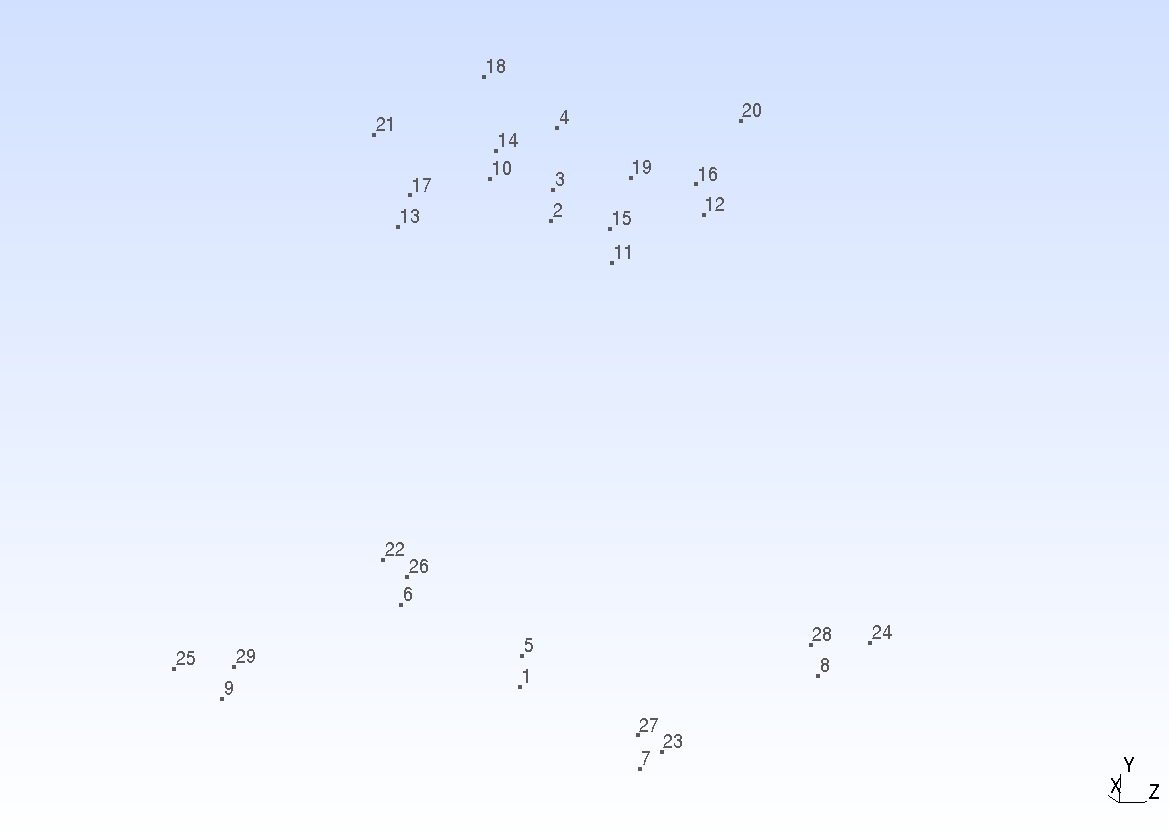
\includegraphics[scale=0.4]{pictures/main_points.png}
	\caption{Опорные точки}
	\label{fig: main_points}
\end{figure}

\begin{figure}[H]
	\center
	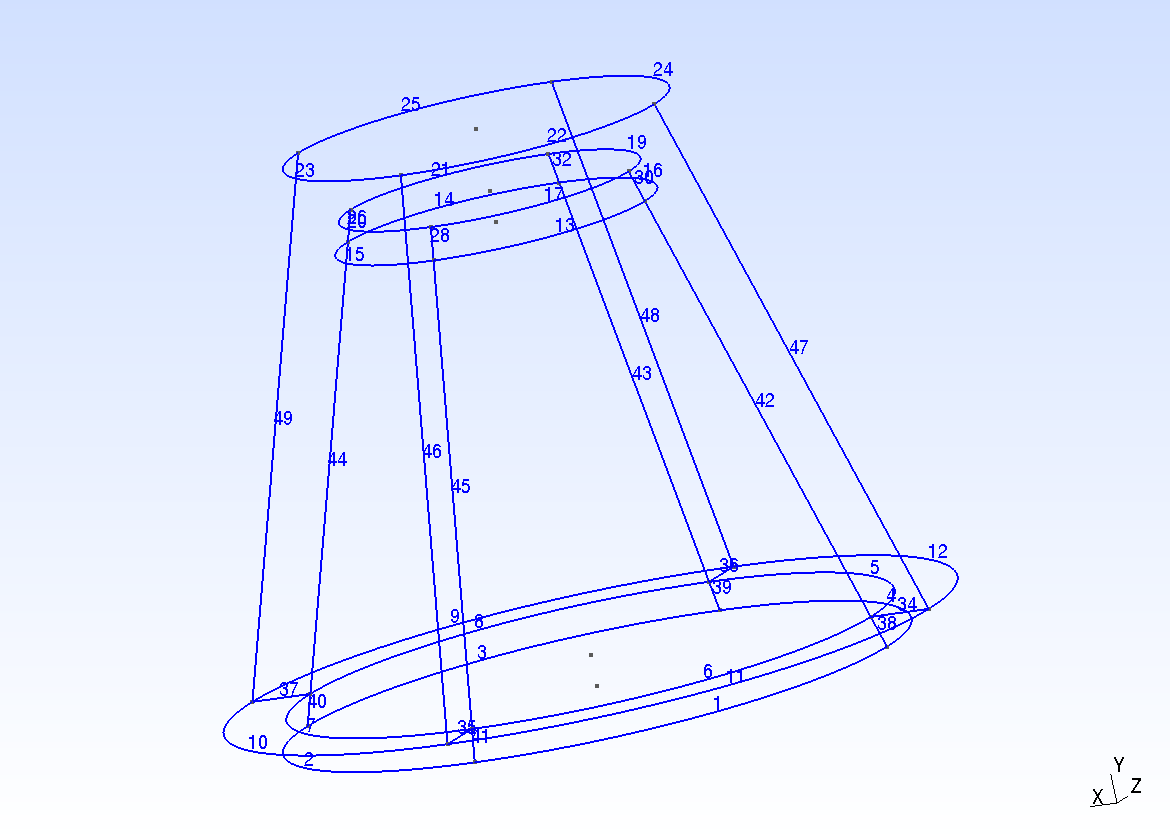
\includegraphics[scale=0.35]{pictures/skeleton.png}
	\caption{Каркас области}
	\label{fig: skeleton}
\end{figure}


\begin{figure}[H]
	\center
	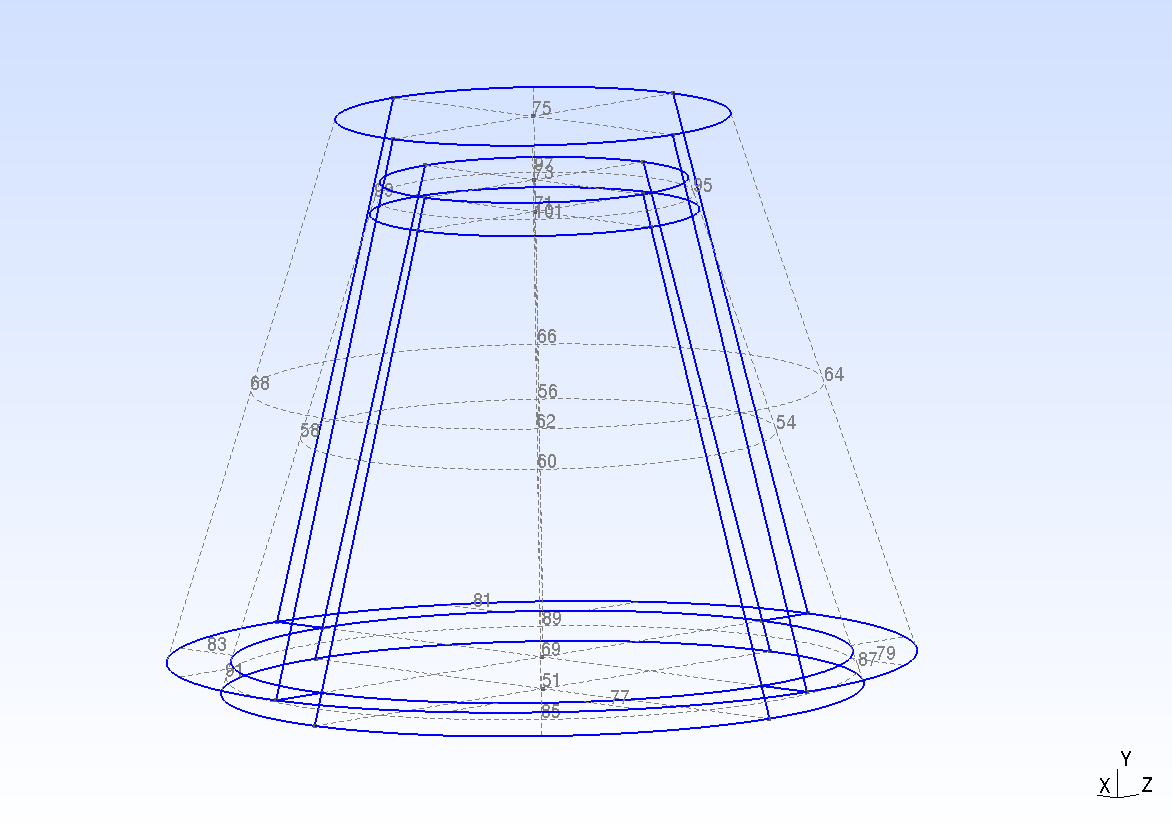
\includegraphics[scale=0.35]{pictures/surfaces.png}
	\caption{Поверхности}
	\label{fig: surfaces}
\end{figure}

\begin{figure}[H]
	\center
	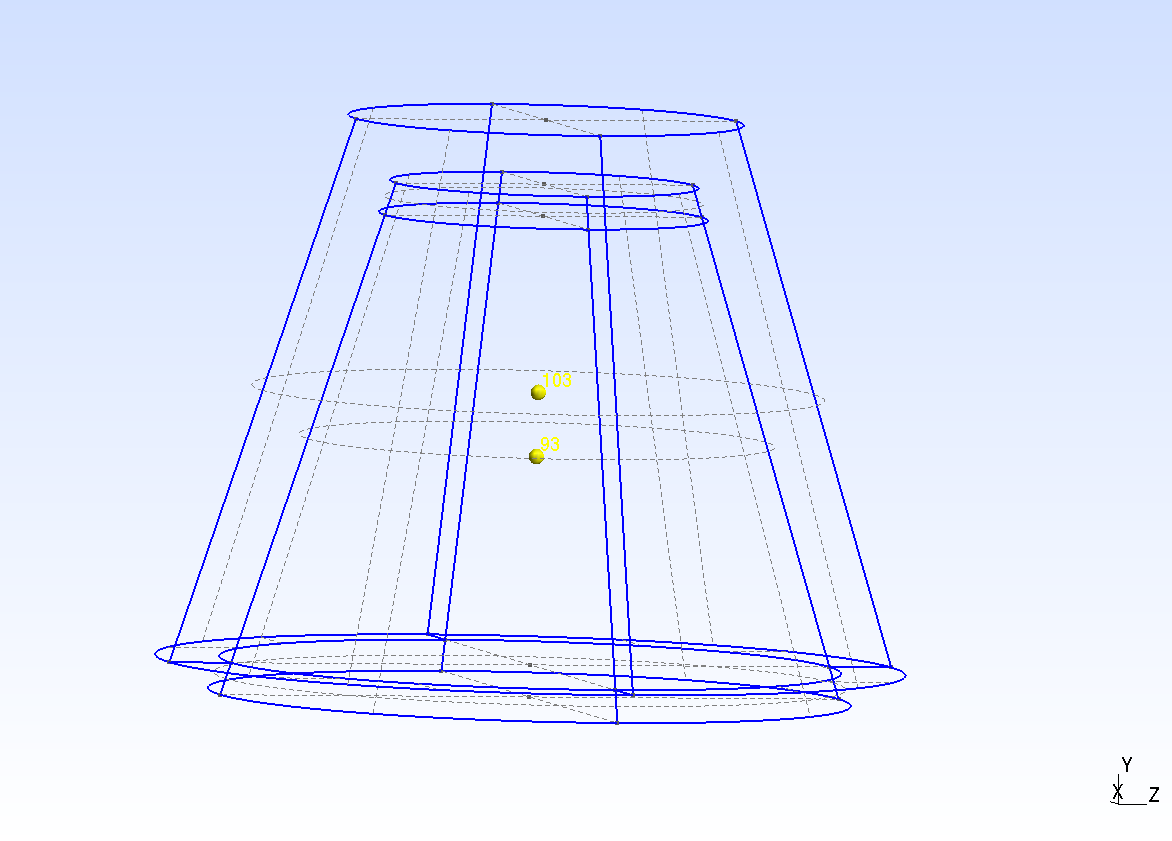
\includegraphics[scale=0.4]{pictures/volumes.png}
	\caption{Области}
	\label{fig: volumes}
\end{figure}

Также мы будем использовать функцию \enquote{пометки} поверхностей и областей пакета \texttt{Gmsh}. Отметить поверхности необходимо, чтобы она была выделена при генерации сетки (ячейки, грани которых принадлежат этой области, будут отмечены также индексом этой области), чтобы после была возможность выделить поверхности из всей сетки и задать отдельные условия для нее.

Пример пометки поверхностей:
\begin{lstlisting}
surf1 = 1;
surf2 = 2;
surf3 = 3;
Physical Surface(surf1) = {75};
Physical Surface(surf2) = {51};
Physical Surface(surf3) = {58, 56, 54, 60};
\end{lstlisting}

\subsection{Генерация сетки}

Следующим шагом после формирования области является генерация сетки.

\texttt{Gmsh} позволяет генерировать 1D, 2D, 3D сетки с помощью 
GUI либо консольных команд, имеет некоторые инструменты
для настройки построенной сетки, различные режимы ее отображения
и, разумеется, предоставляет возможность сохранять построенную сетку в файл.

Для построения сетки и последующим преобразованием его к 
формату, который 
мы будем использовать в дальнейшем, используется следующий  
скрипт на языке \texttt{Python}:

\begin{lstlisting}
import os
os.system("gmsh -3 -format msh ./domain/final.geo")
os.system("dolfin-convert ./domain/final.msh ./domain/mesh.xml")
\end{lstlisting}

В итоге будем иметь несколько \textbf{.xml} файлов с описанием
сетки на нашей области.

На рисунке \ref{fig: mesh_display}
проиллюстрирована наша сетка в режиме отображения границ
поверхностей ячеек и в режиме отображения самих ячеек со срезом.

\begin{figure}[H]
	\begin{subfigure}[h]{0.5\textwidth}
		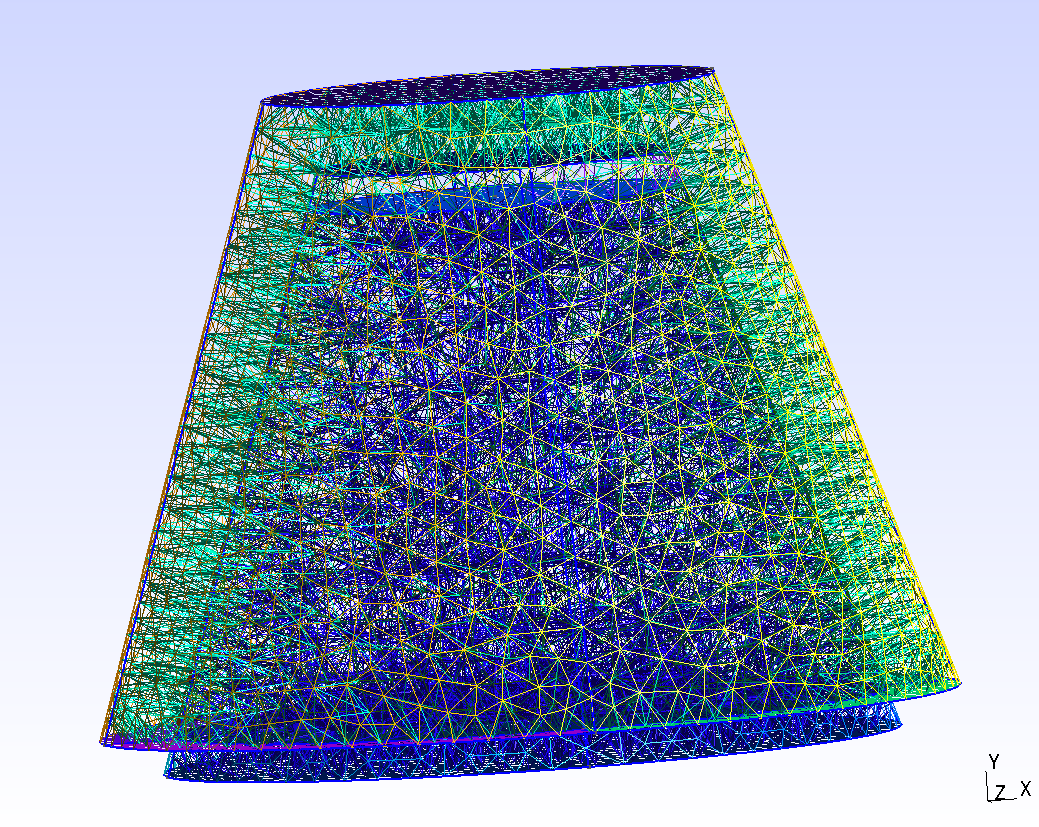
\includegraphics[scale=0.23]{pictures/mesh_surfaces_edges_full.png}
	\end{subfigure}
	\begin{subfigure}[h]{0.5\textwidth}
		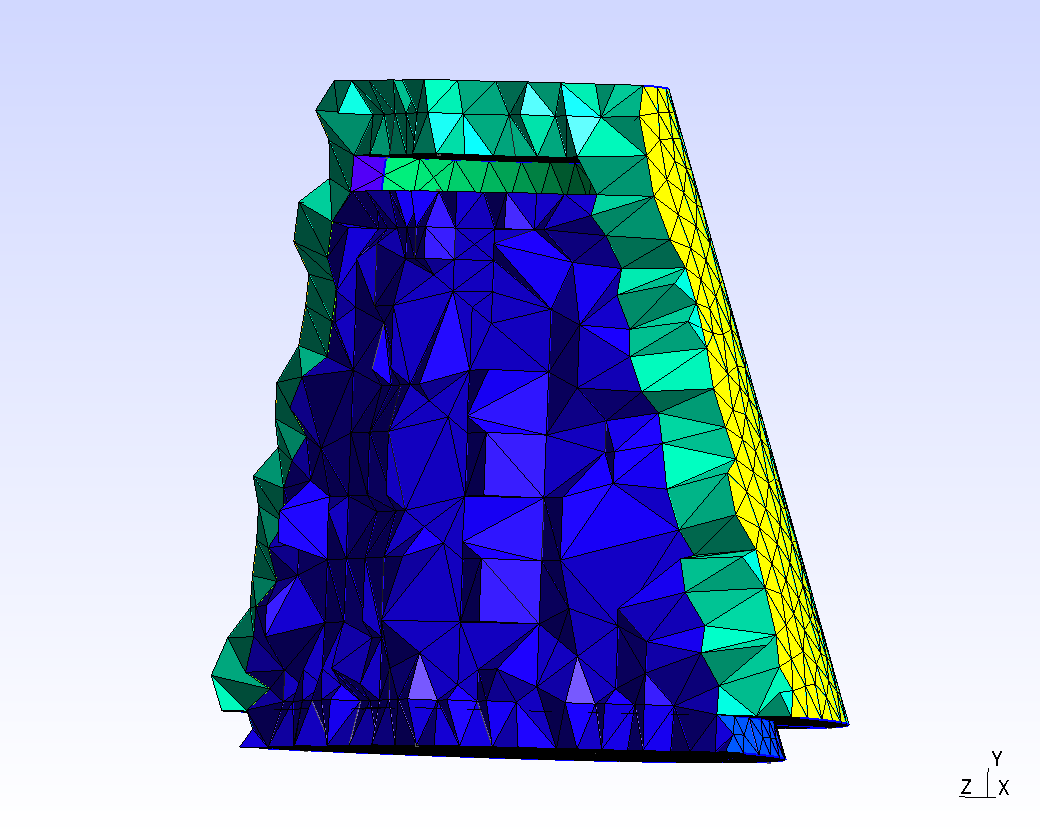
\includegraphics[scale=0.23]{pictures/mesh_volumes_slice.png}
	\end{subfigure}
	\caption{Примеры визуализации сетки (границы поверхностей элементов сетки и срез с отображением самих ячеек)}
	\label{fig: mesh_display}
\end{figure}


\section{Описание процесса численного эксперимента}

\textbf{Чтение параметров}

Для начала прочитаем из файла параметров, собственно, параметры:
\begin{lstlisting}
param_file = File("problem.xml")
params = Parameters("parameters")
param_file >> params
info(params, True)
\end{lstlisting}

Командой \texttt{info} выведем их в консоль. 

\textbf{Вычисление модулей упругости}

Достанем из параметров значения прилагаемой нагрузки и
коэффициенты Юнга и Пуассона, по которым вычислим коэффициенты Ламе (\ref{eq: young_puasson}):
\begin{lstlisting}
nu_values = np.array([params['coefficients']['Poisson']['1'],
params['coefficients']['Poisson']['2']])
E_values = np.array([params['coefficients']['Young']['1'],
params['coefficients']['Young']['2']])
mu_values = E_values / (2.0 * (1.0 + nu_values))
lmbd_values = E_values * nu_values / \
    ((1.0 + nu_values) * (1.0 - 2.0 * nu_values))
\end{lstlisting}
Используемые значения коэффициентов Юнга и Пуассона характерны для никель-хромовой стали.

\textbf{Чтение нагрузки}

Достанем из параметров значения придаваемой нагрузки:
\begin{lstlisting}
g_value = [params['pressure']['g']['x'],
           		  params['pressure']['g']['y'],
           	 	  params['pressure']['g']['z']]
\end{lstlisting}

\textbf{Чтение сетки и областей}

Прочитаем сгенерированную сетку, а также отдельно ячейки каждой подобласти и каждой части границы. Для поверхностей ячеек вычислим вектор нормали:
\begin{lstlisting}
mesh = Mesh(params['mesh']['path'])
subdomains = MeshFunction("size_t", mesh, params['mesh']['domains'])
boundaries = MeshFunction("size_t", mesh, params['mesh']['bounds'])
n = FacetNormal(mesh)
\end{lstlisting}

\textbf{Применение модулей упругости}

Установим каждой из областей коэффициенты Ламе:
\begin{lstlisting}
V0 = FunctionSpace(mesh, 'DG', 0)
mu = Function(V0)
lmbda = Function(V0)

help = np.asarray(subdomains.array(), dtype=np.int32)
mu.vector()[:] = np.choose(help, mu_values)
lmbda.vector()[:] = np.choose(help, lmbd_values)
\end{lstlisting}

\textbf{Задание пространства конечных элементов, нагрузки и перемещений}

Зададим пространство используемых конечных элементов,
функции $\textbf{g}$ и $\textbf{u}_0$, а также триальную и тестовую
функции $\textbf{u}$ и $\textbf{v}$:
\begin{lstlisting}
V = VectorFunctionSpace(mesh, "CG", 1)
g = Expression((str(g_value[0]), str(g_value[1]), str(g_value[2])))
u_0 = Expression(("0.0", "0.0", "0.0"))
u = TrialFunction(V)
v = TestFunction(V)
\end{lstlisting}

\textbf{Граничные условия}

Для границы $\Gamma_1$ зададим условия типа Дирихле:
\begin{lstlisting}
bc = DirichletBC(V, u_0, boundaries, 2)
\end{lstlisting}

\textbf{Области интегрирования}

Объявим области для интегрирования по области $\Omega$ и по границе
$\partial\Omega$:
\begin{lstlisting}
dx = Measure('dx', domain=mesh, subdomain_data=subdomains)
ds = Measure('ds', domain=mesh, subdomain_data=boundaries)
\end{lstlisting}

\textbf{Задание тензора напряжений и линейной и билинейной форм}

Зададим тензор напряжений как функцию и вычислим линейную и билинейную формы:
\begin{lstlisting}
def sigma(v, mu, lmb):
    return 2.0 * mu * sym(grad(v)) + lmb * tr(sym(grad(v))) * \
        Identity(v.cell().topological_dimension())
a = inner(sigma(u, mu, lmbda), sym(grad(v))) * dx(0) + \
    inner(sigma(u, mu, lmbda), sym(grad(v))) * dx(1)
L = inner(g, v) * ds(1)
\end{lstlisting}

\textbf{Вычисление приближенного решения}

Запустив функцию \texttt{solve()} для нашей задачи,
\begin{lstlisting}
u = Function(V)
solve(a == L, u, bc)

displ_file = File(params['results']['displacement'])
displ_file << u
\end{lstlisting}
мы найдем вектор упругих деформаций для каждой точки области.

\textbf{Вычисление смещенной сетки}

\begin{lstlisting}
mesh.move(u)
newmesh_file = File("./results/mesh.pvd")
newmesh_file << mesh
\end{lstlisting}

\textbf{Вычисление напряжений}

\begin{lstlisting}
W = TensorFunctionSpace(mesh, "CG", 1)
stress = Function(W)
stress = project(sigma(u, mu, lmbda), W)

stress_file = File(params['results']['stress'])
stress_file << stress
\end{lstlisting}

\textbf{Нормальные и тангенциальные составляющие напряжений}

\begin{lstlisting}
n = FacetNormal(mesh)
T = dot(-s, n)

Tn = inner(T, n)  # скаляр
Tt = T - Tn * n   # вектор

scalar = FunctionSpace(mesh, "DG", 0)
vector = VectorFunctionSpace(mesh, "DG", 1)
v = TestFunction(scalar)
w = TestFunction(vector)

normal_stress = Function(scalar)
shear_stress = Function(vector)
Ln = (1 / FacetArea(mesh)) * v * Tn * ds
Lt = (1 / FacetArea(mesh)) * inner(w, Tt) * ds
assemble(Ln, tensor=normal_stress.vector())
assemble(Lt, tensor=shear_stress.vector())
\end{lstlisting}

\textbf{Вычисление отношений на границе областей}

\begin{lstlisting}
k = Tn - 0.3 * sqrt(dot(Tt, Tt))
rel = Function(scalar)
rel_projection = (1 / FacetArea(mesh)) * v * k * ds
assemble(rel_projection, tensor=rel.vector())

rel_file = File(params['results']['destination']['relation'])
rel_file << rel

normal_stress_file = File(params['results']['destination']['normal_stress'])
normal_stress_file << normal_stress
shear_stress_file = File(params['results']['destination']['shear_stress'])
shear_stress_file << shear_stress
\end{lstlisting}

Полный листинг кода приведен в приложении А.

\section{Визуализация и анализ результатов}

\texttt{Paraview} предоставляет множество возможностей
для визуализации результатов.
Покажем, как выглядят некоторые из рассчитанных величин.
(рисунки \ref{fig: result_push_displacement_slice} -- 
\ref{fig: result_push_shear_stress_partial}).

\begin{figure}[H]
	\center
	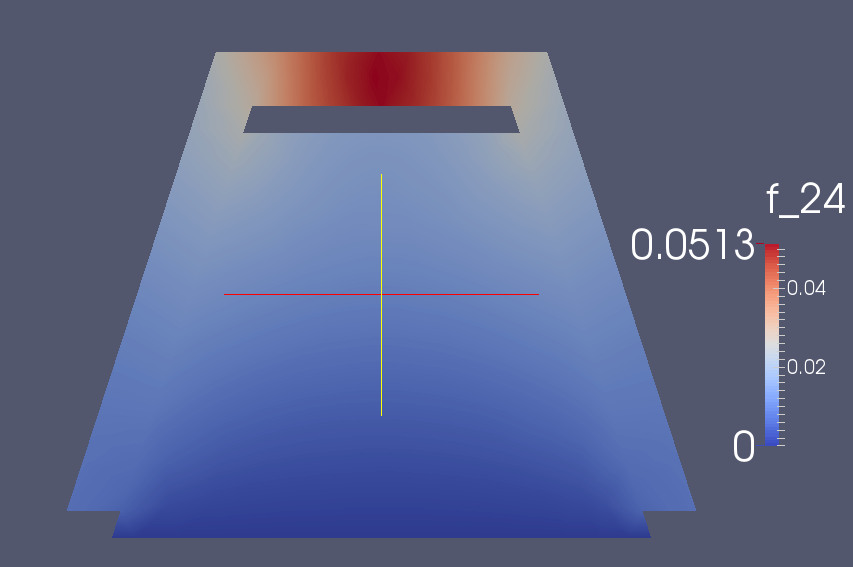
\includegraphics[scale=0.4]{pictures/result_push_displacement_slice.png}
	\caption{Модуль перемещений деформированного тела (разрез)}
	\label{fig: result_push_displacement_slice}
\end{figure}

\begin{figure}[H]
	\center
	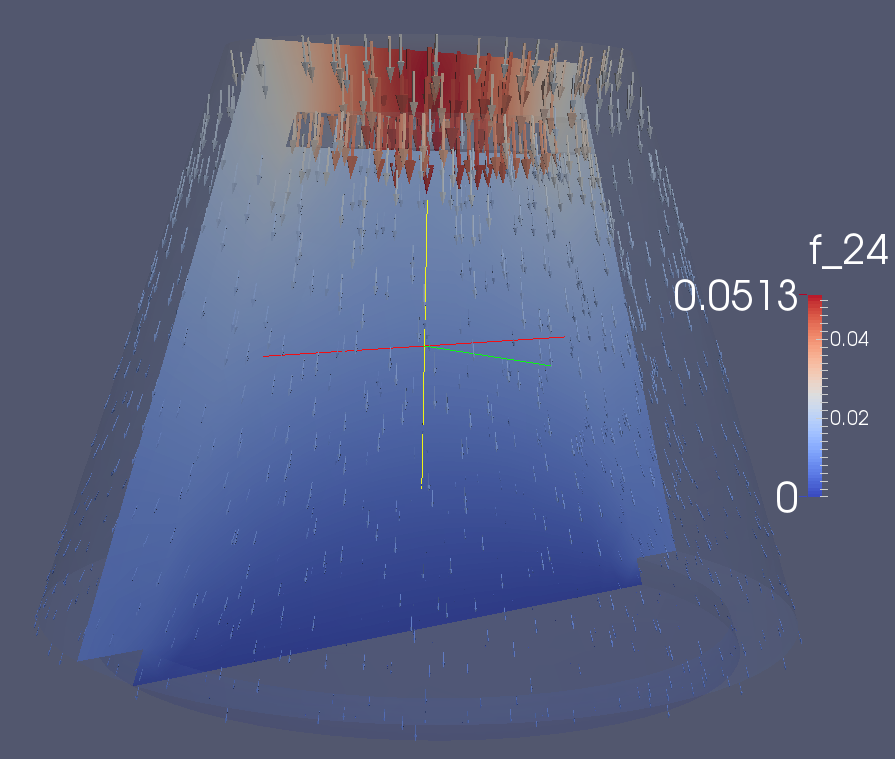
\includegraphics[scale=0.5]{pictures/result_push_displacement_glyph.png}
	\caption{Перемещения деформированного тела (glyph)}
	\label{fig: result_push_displacement_glyph}
\end{figure}

\begin{figure}[H]
	\center
	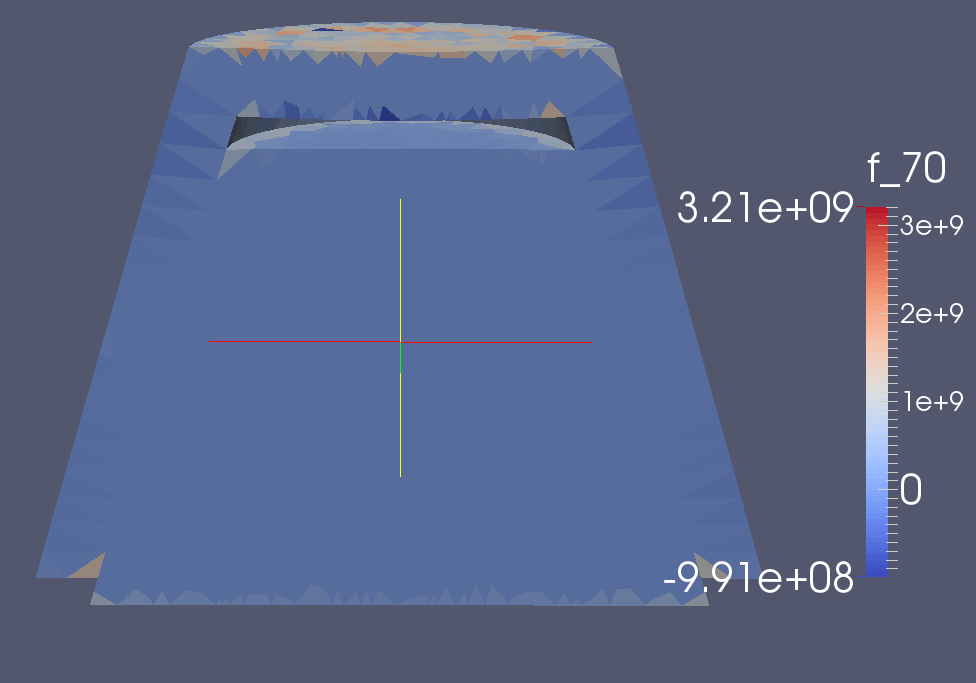
\includegraphics[scale=0.35]{pictures/result_push_normal_stress_slice.png}
	\caption{Нормальные напряжения деформированного тела}
	\label{fig: result_push_normal_stress_slice}
\end{figure}

\begin{figure}[H]
	\center
	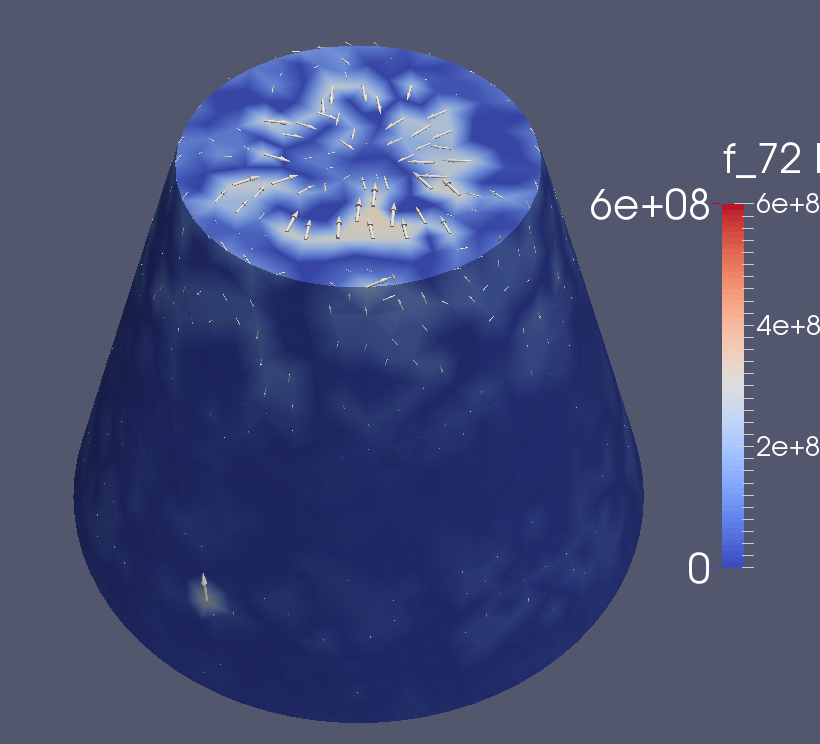
\includegraphics[scale=0.45]{pictures/result_push_shear_stress_full.png}
	\caption{Тангенциальные напряжения деформированного тела (внешняя поверхность)}
	\label{fig: result_push_shear_stress_full}
\end{figure}

\begin{figure}[H]
	\center
	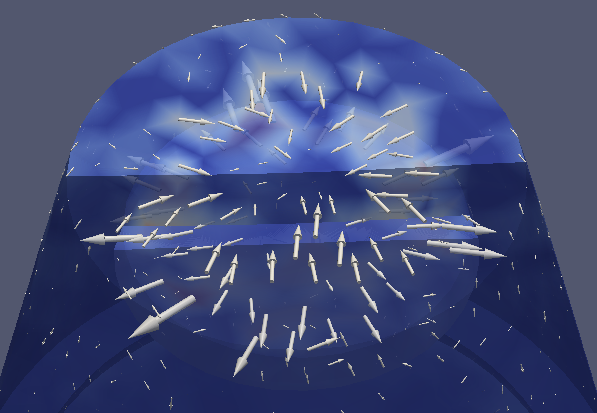
\includegraphics[scale=0.55]{pictures/result_push_shear_stress_partial.png}
	\caption{Тангенциальные напряжения  внутри деформированного тела}
	\label{fig: result_push_shear_stress_partial}
\end{figure}

Далее проанализируем силу удержания для всего набора углов 
($4^{\circ}$ - $12^{\circ}$), прикладывая давление 
порядка $4\cdot10^8$ Па. Данная величина в несколько раз
превышает 
силу давления, которую создают человеческие челюсти при
жевании.

Будем отображать те ячейки, которые находятся вблизи 
границы сопряжения областей и на которых вычисленная сила
$f_h$ имеет значение, большее -- это означает, что на этой 
ячейке возникла сила удержания.

Оценивая количество и плотность таких ячеек, можно оценить,
насколько тот или иной угол эффективен для телескопических 
конусовидных коронок.

Результаты представлены на рисунках \ref{fig: push4-4deg} -- 
\ref{fig: push4-12deg}.

\begin{figure}[H]
	\center
	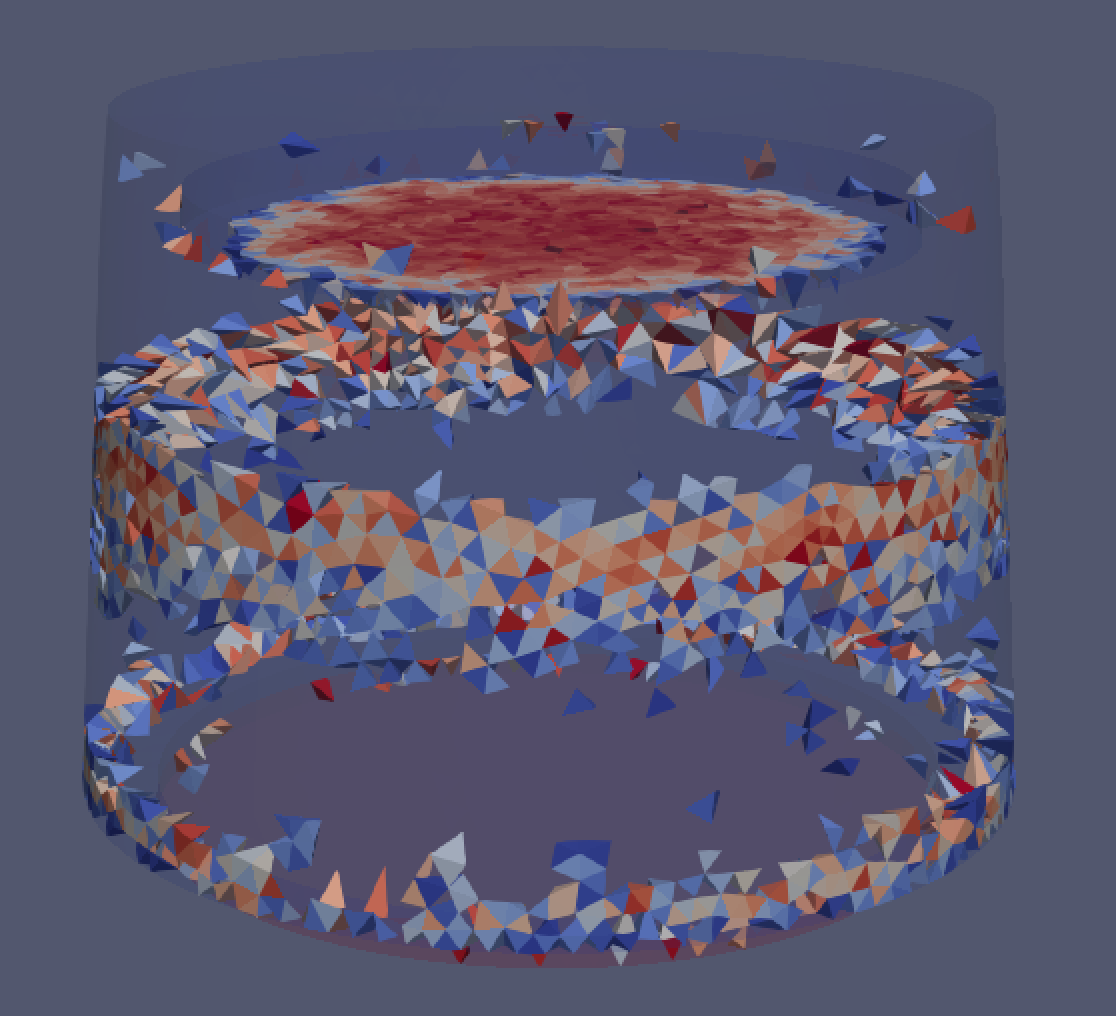
\includegraphics[scale=0.6]{pictures_diploma/push4-4deg.png}
	\caption{Ячейки, на которых возникла сила удержания ($4^{\circ}$)}
	\label{fig: push4-4deg}
\end{figure}

\begin{figure}[H]
	\center
	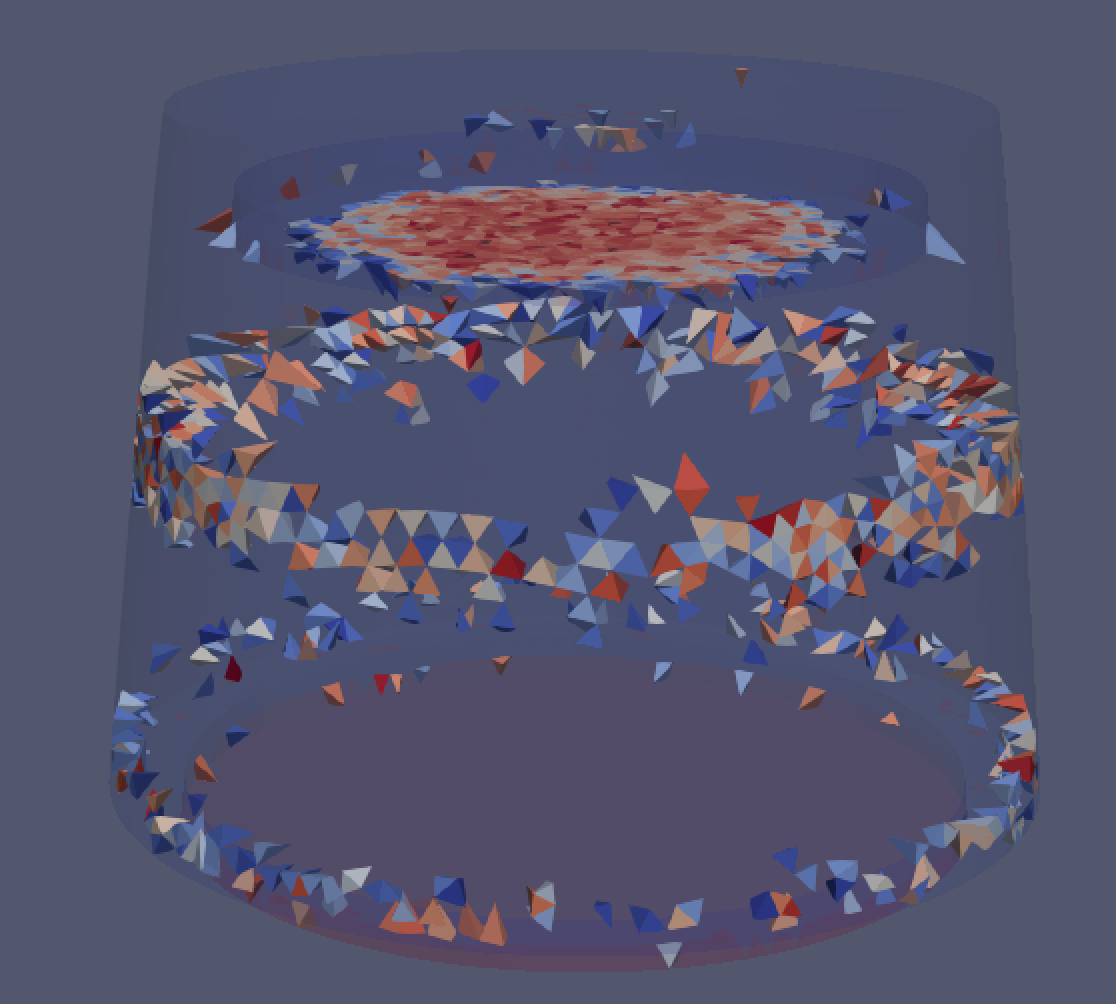
\includegraphics[scale=0.6]{pictures_diploma/push4-6deg.png}
	\caption{Ячейки, на которых возникла сила удержания ($6^{\circ}$)}
	\label{fig: push4-6deg}
\end{figure}

\begin{figure}[H]
	\center
	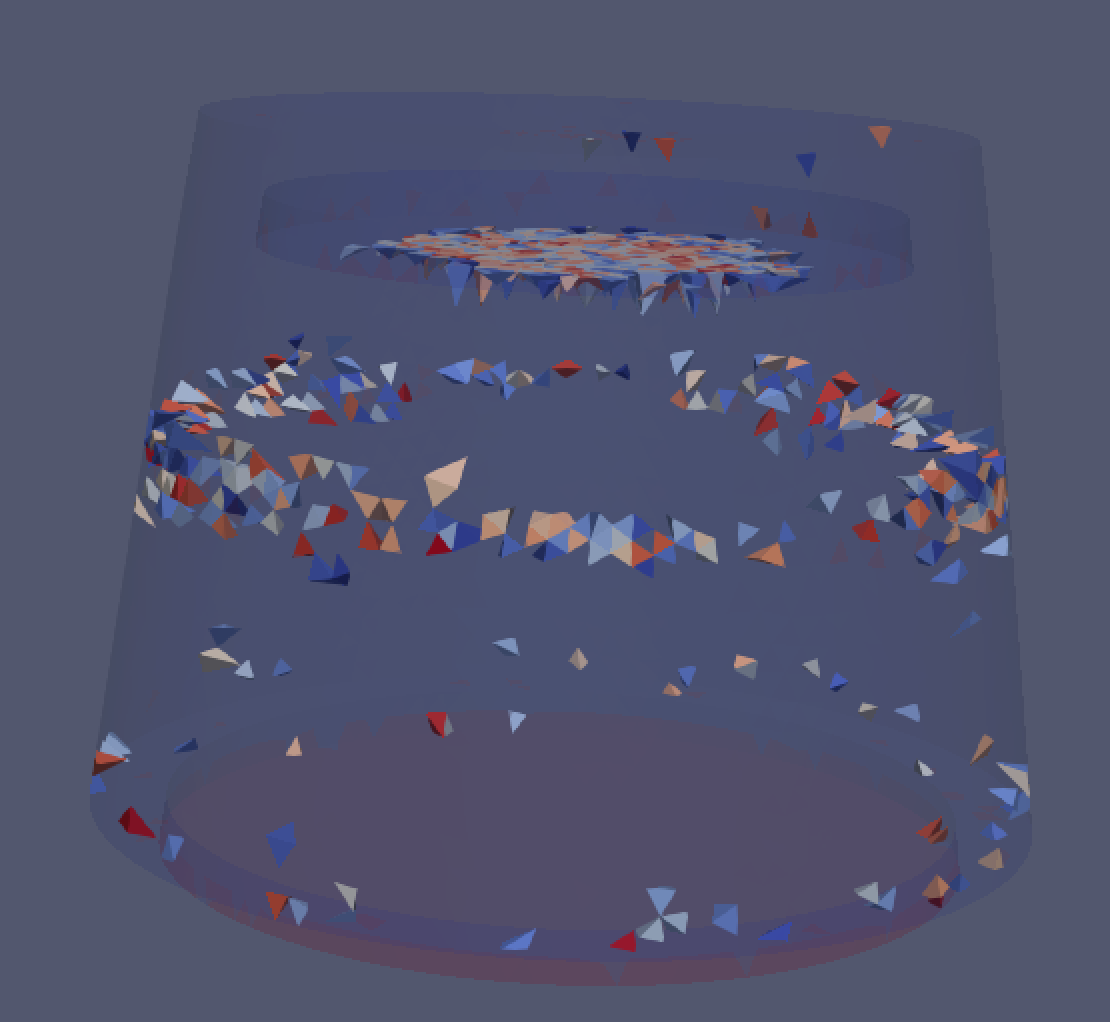
\includegraphics[scale=0.6]{pictures_diploma/push4-8deg.png}
	\caption{Ячейки, на которых возникла сила удержания ($8^{\circ}$)}
	\label{fig: push4-8deg}
\end{figure}

\begin{figure}[H]
	\center
	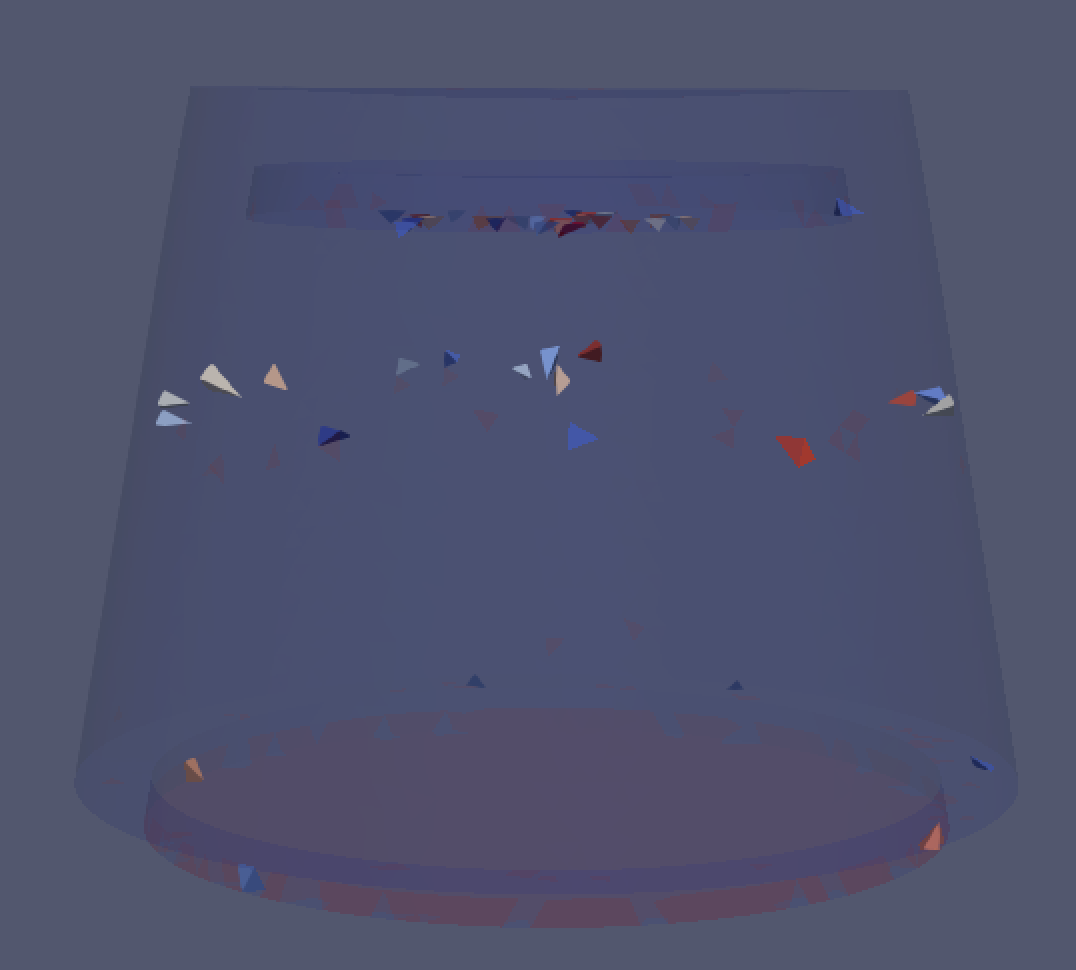
\includegraphics[scale=0.6]{pictures_diploma/push4-10deg.png}
	\caption{Ячейки, на которых возникла сила удержания ($10^{\circ}$)}
	\label{fig: push4-10deg}
\end{figure}

\begin{figure}[H]
	\center
	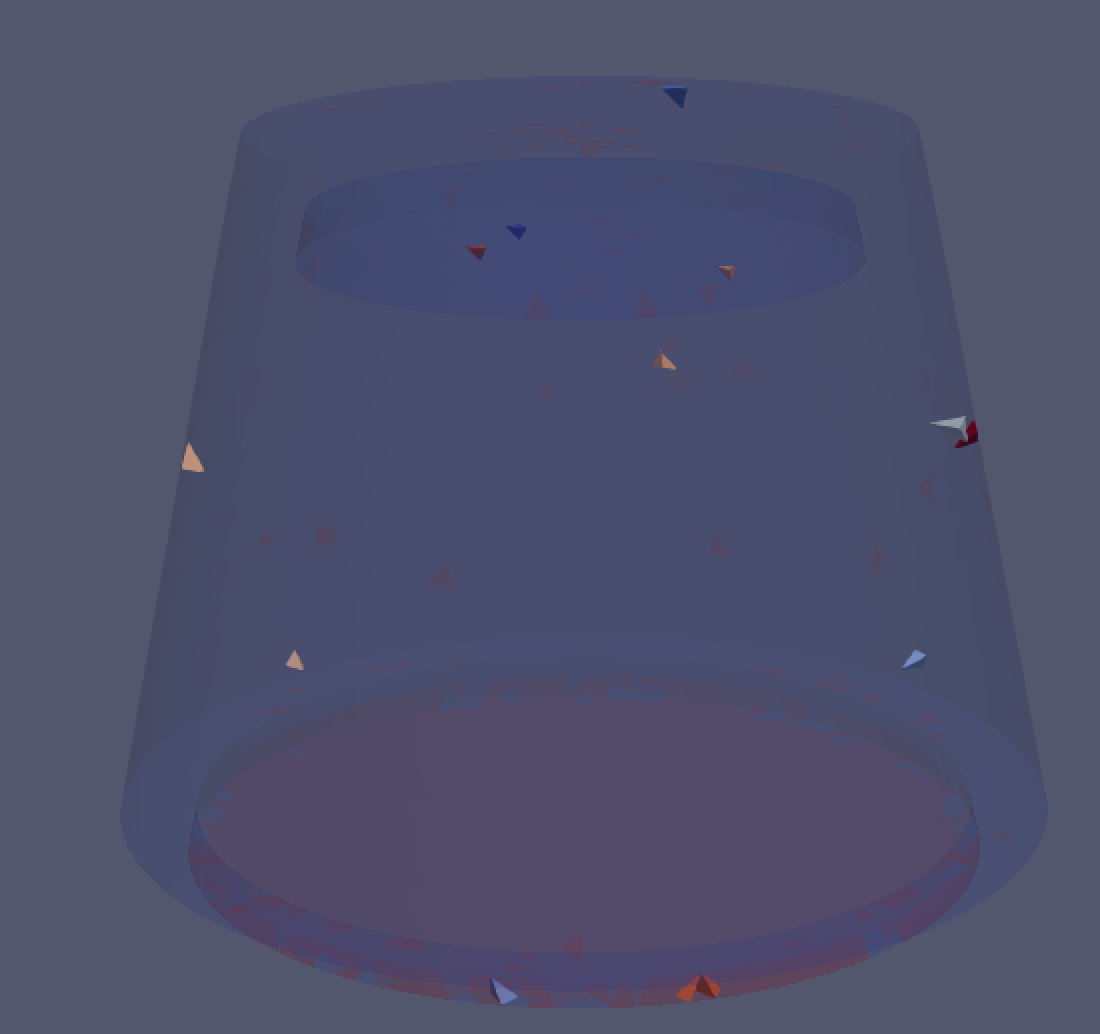
\includegraphics[scale=0.6]{pictures_diploma/push4-12deg.png}
	\caption{Ячейки, на которых возникла сила удержания ($12^{\circ}$)}
	\label{fig: push4-12deg}
\end{figure}

В таблице \ref{tab: table1} для всех вариантов нагрузок и 
углов представлены максимальные значения возникшей силы 
удержания:

\begin{table}[H]
\captionsetup{width=1.5\textwidth}
\centering
\caption{Максимальные значения силы удержания,  
Па $\cdot 10^7$}
\begin{tabular}{l*{6}{c}r}
Нагрузка, Па              & $4^{\circ}$ & $6^{\circ}$ & $8^{\circ}$ & $10^{\circ}$ & $12^{\circ}$ \\
\hline
$1 \cdot 10^8$ 	& 7.1 & 6 & 4.1 & 3.2 & 3  \\
$2 \cdot 10^8$     & 14.1 & 12.4 & 8.4 & 6.1 & 6  \\
$4 \cdot 10^8$     & 28 & 24.2 & 17.2 & 12.2 &  10.9  \\
$8 \cdot 10^8$     & 60.6 & 50.4 & 36.1 & 25.3 &  22.3  \\
\end{tabular}

\label{tab: table1}
\end{table}

Как видно из представленных выше результатов, величина 
угла наклона образующей конуса обратно пропорциональна величине возникающей силы удержания. На практике, не 
рекомендуется использовать углы больше $6^{\circ}$ для 
телескопических конусовидных коронок.

\newpage
\phantomsection
\begin{center}
\addcontentsline{toc}{section}{ЗАКЛЮЧЕНИЕ}
	\Large{\textbf{ЗАКЛЮЧЕНИЕ}}
\end{center}

Основные результаты данной дипломной работы следующие:
\begin{enumerate}
\item  Для решения граничной задачи теории упругости в 
области сложной формы построен численный метод,
основанный на методе конечных элементов

\item Проведено моделирование конструкции телескопических 
конусовидных коронок. Для моделирования была разработана
программа на языке \texttt{Python}. Для реализации 
вычислений использовался пакет для научных вычислений
\texttt{FEniCS}.

\item На основе моделирования проведена оценка влияния 
геометрических параметров коронки на силу удержания.
В целом установлено, что для конусовидных коронок не 
стоит выбирать угол больше $6^{\circ}$, т.к. для больших углов 
сила удержания резко уменьшается.

\end{enumerate}


\newpage
\phantomsection
\renewcommand{\bibname}{\Large{СПИСОК ИСПОЛЬЗОВАННЫХ ИСТОЧНИКОВ}}
\addcontentsline{toc}{section}{СПИСОК ИСПОЛЬЗОВАННЫХ ИСТОЧНИКОВ}
\begin{thebibliography}{9}

	\bibitem{finite_element_method}
			Hughes Thomas J. R.,
			{The finite element method: linear static and dynamic finite element analysis} /
			Hughes Thomas J. R., -- Dover Publications, 2012. -- 704 c.
	\bibitem{math_elasticity_theory}
			Сьярле Ф.,
			{Математическая теория упругости} /
			Сьярле Ф. Перевод с англ. -- Г. А. Иосифьяна ; под ред. О. А. Олейник, -- Москва: Мир, 1992. -- 472 c.
	\bibitem{fenics_book}
			Logg A.,
			{Automated Solution of Differential Equations by the Finite Element Method. The FEniCS book} /
			Anders Logg, Kent-Andre Mardal, Garth N. Wells, -- Berlin: Shpringer, 2011. -- 720 c.
\end{thebibliography}



\newpage
	\phantomsection
\addcontentsline{toc}{section}{ПРИЛОЖЕНИЕ А}
\addcontentsline{toc}{section}{Листинг программы для решения задачи}
\begin{center}
	\begin{flushright}
		\Large{\textbf{ПРИЛОЖЕНИЕ А}}\\
	\end{flushright}
	\textbf{Листинг программы для решения задачи}
\end{center}

\lstinputlisting[basicstyle=\tiny, backgroundcolor = \color{white}, title=Data, language=XML]{../problem-template.xml}
\lstinputlisting[basicstyle=\small, backgroundcolor = \color{white}, title=Main]{../main.py}
\lstinputlisting[basicstyle=\small, backgroundcolor = \color{white}, title=Elasticity]{../elasticity.py}
\lstinputlisting[basicstyle=\small, backgroundcolor = \color{white}, title=Mesh]{../meshgen.py}

\end{document}